\documentclass[11pt,letterpaper]{article}

% -----------------------------------------------------------------------------
% Documento autocontenido para TeX Live y LaTeX Workshop.
% Las imagenes pendientes estan indicadas con comentarios y marcadores visibles.
% El archivo compila sin necesidad de agregar imagenes externas.
% -----------------------------------------------------------------------------

\usepackage[utf8]{inputenc}
\usepackage[T1]{fontenc}
\usepackage[spanish,es-nodecimaldot]{babel}
\usepackage{lmodern}
\usepackage{microtype}
\usepackage[letterpaper,margin=2.15cm]{geometry}
\usepackage[table]{xcolor}
\usepackage{graphicx}
\usepackage{booktabs}
\usepackage{tabularx}
\usepackage{array}
\usepackage{enumitem}
\usepackage{tikz}
\usetikzlibrary{arrows.meta,positioning,shapes.geometric,fit}
\usepackage{titlesec}
\usepackage{fancyhdr}
\usepackage{hyperref}

\definecolor{azulaws}{HTML}{1D4ED8}
\definecolor{azulclaro}{HTML}{DBEAFE}
\definecolor{verdeclinica}{HTML}{047857}
\definecolor{verdeclaro}{HTML}{D1FAE5}
\definecolor{gristexto}{HTML}{334155}
\definecolor{grisborde}{HTML}{CBD5E1}
\definecolor{grisfondo}{HTML}{F8FAFC}

\hypersetup{
  colorlinks=true,
  linkcolor=azulaws,
  urlcolor=azulaws,
  pdftitle={Arquitectura de datos para la Clinica del Sur},
  pdfauthor={Trabajo grupal - Modulo V}
}

\titleformat{\section}
  {\large\bfseries\color{black}}
  {\thesection.}{0.55em}{}
\titleformat{\subsection}
  {\normalsize\bfseries\color{black}}
  {\thesubsection.}{0.55em}{}
\titlespacing*{\section}{0pt}{1.1em}{0.45em}
\titlespacing*{\subsection}{0pt}{0.8em}{0.3em}

\setlength{\parindent}{0pt}
\setlength{\parskip}{0.45em}
\renewcommand{\arraystretch}{1.23}
\setlist[itemize]{leftmargin=1.4em,itemsep=0.15em,topsep=0.2em}

\pagestyle{fancy}
\fancyhf{}
\fancyhead[L]{\small Clinica del Sur}
\fancyhead[R]{\small Arquitectura de datos en AWS}
\fancyfoot[C]{\thepage}
\renewcommand{\headrulewidth}{0.3pt}

\newcolumntype{Y}{>{\raggedright\arraybackslash}X}
\newcolumntype{C}[1]{>{\centering\arraybackslash}p{#1}}

\newcommand{\marcadorimagen}[2]{%
  \begin{center}
    \fcolorbox{grisborde}{grisfondo}{%
      \parbox[c][#1][c]{0.92\linewidth}{%
        \centering\color{gristexto}\small\textbf{Imagen pendiente}\\[0.35em]
        #2
      }%
    }
  \end{center}
}

\begin{document}

\begin{titlepage}
  \centering



  \vspace{0.7cm}
  {\large\bfseries UNIVERSIDAD MAYOR DE SAN ANDRES\par}
  \vspace{0.25cm}
  {\normalsize POSTGRADO EN INFORMATICA\par}
  {\normalsize Maestria en Inteligencia Artificial y Data Science\par}
  {\normalsize para la Transformacion de Negocios\par}
    \vspace{0.35cm}

    % IMAGEN PENDIENTE: copiar el logotipo institucional a
  % latex-workshop/figures/logo_postgrado.png y sustituir el marcador por:
  
\includegraphics[width=7cm]{figures/logo_postgrado.png}

  {\LARGE\bfseries Propuesta de arquitectura de datos para la Clinica del Sur\par}
  \vspace{0.35cm}
  {\large Caso ficticio con Amazon RDS, Amazon S3 y AWS IAM\par}

  \vfill
  \begin{tabular}{@{}ll@{}}
    \textbf{Modulo:} & V -- Ecosistema de Negocios y Arquitecturas de Datos \\
    \textbf{Docente:} & Ronny Bazan Antequera, Ph.D. \\
    \textbf{Integrantes:} & Callisaya Genesis \\
      & Alave Sanjines Cristhian Rodrigo \\
      & Loza Ramirez Samuel \\
      & Liceth Quispe Apaza \\
  \end{tabular}

  \vfill
  {La Paz, Bolivia -- 1 de octubre del 2026\par}
\end{titlepage}

\section{Negocio y estrategia}

\subsection{Descripcion del negocio}

El caso de estudio corresponde a una clinica que brinda servicios de atencion medica en
diferentes especialidades. Para desarrollar sus actividades, la clinica genera y administra
informacion relacionada con pacientes, medicos, especialidades, citas, atenciones, consultas y
pagos.

Debido a la cantidad de informacion generada diariamente, es importante contar con una forma
organizada de almacenar y gestionar estos datos, de manera que puedan utilizarse posteriormente
para realizar analisis y apoyar la toma de decisiones.

\subsection{Problema o necesidad}

La clinica necesita mejorar la organizacion y el manejo de la informacion que genera durante sus
actividades. Al tener los datos distribuidos en diferentes registros o archivos, puede resultar
dificil obtener informacion actualizada sobre la atencion de los pacientes y el funcionamiento de
los servicios.

Entre las principales necesidades se encuentran conocer que especialidades tienen mayor demanda,
realizar un seguimiento de las citas atendidas y canceladas, y analizar la cantidad de atenciones
realizadas.

Por este motivo, se propone implementar una arquitectura de datos en AWS que permita centralizar,
almacenar y organizar la informacion de la clinica, facilitando su consulta y analisis.

\subsection{Objetivo estrategico}

Mejorar la gestion de las citas y la atencion de los pacientes mediante el analisis de los datos
de la clinica, con el proposito de optimizar los servicios y el uso de los recursos disponibles.

\section{Datos y Amazon RDS}

La Clinica del Sur utilizara Amazon RDS para almacenar los datos estructurados relacionados con la
administracion de pacientes, medicos, especialidades, consultorios, citas y atenciones. Las tablas
estaran relacionadas mediante claves primarias y foraneas, lo que permitira organizar la
informacion y realizar consultas para calcular los KPI definidos en el punto 3.

\subsection{Tipos de datos}

\begin{table}[htbp]
  \centering
  \small
  \caption{Tipos de datos relevantes para la clinica}
  \begin{tabularx}{\textwidth}{@{}C{1.1cm}p{4.2cm}Y@{}}
    \toprule
    \rowcolor{azulclaro}
    \textbf{N.} & \textbf{Tipo de dato} & \textbf{Descripcion} \\
    \midrule
    1 & Datos de pacientes & Informacion basica para identificar y contactar al paciente. \\
    2 & Datos de medicos & Informacion de los profesionales que atienden en la clinica. \\
    3 & Datos de especialidades & Informacion de las especialidades medicas disponibles. \\
    4 & Datos de citas & Informacion sobre las citas programadas y su estado. \\
    5 & Datos de atenciones & Informacion sobre las atenciones realizadas a partir de una cita. \\
    \bottomrule
  \end{tabularx}
\end{table}

\subsection{Informacion que se almacenara en RDS}

Amazon RDS almacenara la informacion estructurada de la clinica: pacientes, medicos,
especialidades, consultorios, citas y atenciones. Estos datos se organizaran en tablas relacionadas
para registrar y consultar las operaciones de la clinica. La informacion de RDS servira como
fuente principal para calcular los KPI, mientras que los documentos, imagenes y reportes se
almacenaran en Amazon S3.

\subsection{Tablas basicas para RDS}

\subsubsection*{PACIENTE}
\begin{center}
\small
\begin{tabularx}{\textwidth}{@{}p{3.2cm}p{3cm}p{2cm}Y@{}}
  \toprule
  \rowcolor{azulclaro}
  \textbf{Campo} & \textbf{Tipo de dato} & \textbf{Clave} & \textbf{Descripcion} \\
  \midrule
  paciente\_id & INT & PK & Identificador unico del paciente. \\
  ci & VARCHAR(20) & UNIQUE & Documento de identidad. \\
  nombre & VARCHAR(100) & -- & Nombre del paciente. \\
  apellido & VARCHAR(100) & -- & Apellido del paciente. \\
  fecha\_nacimiento & DATE & -- & Fecha de nacimiento. \\
  telefono & VARCHAR(20) & -- & Numero de contacto. \\
  email & VARCHAR(150) & -- & Correo electronico. \\
  fecha\_registro & TIMESTAMP & -- & Fecha y hora de registro. \\
  \bottomrule
\end{tabularx}
\end{center}

\subsubsection*{ESPECIALIDAD}
\begin{center}
\small
\begin{tabularx}{\textwidth}{@{}p{3.2cm}p{3cm}p{2cm}Y@{}}
  \toprule
  \rowcolor{azulclaro}
  \textbf{Campo} & \textbf{Tipo de dato} & \textbf{Clave} & \textbf{Descripcion} \\
  \midrule
  especialidad\_id & INT & PK & Identificador de la especialidad. \\
  nombre & VARCHAR(100) & UNIQUE & Nombre de la especialidad. \\
  descripcion & VARCHAR(255) & -- & Descripcion de la especialidad. \\
  estado & VARCHAR(20) & -- & Activa o inactiva. \\
  \bottomrule
\end{tabularx}
\end{center}

\subsubsection*{MEDICO}
\begin{center}
\small
\begin{tabularx}{\textwidth}{@{}p{3.2cm}p{3cm}p{2cm}Y@{}}
  \toprule
  \rowcolor{azulclaro}
  \textbf{Campo} & \textbf{Tipo de dato} & \textbf{Clave} & \textbf{Descripcion} \\
  \midrule
  medico\_id & INT & PK & Identificador unico del medico. \\
  nombre & VARCHAR(100) & -- & Nombre del medico. \\
  apellido & VARCHAR(100) & -- & Apellido del medico. \\
  matricula & VARCHAR(50) & UNIQUE & Matricula profesional. \\
  especialidad\_id & INT & FK & Especialidad del medico. \\
  estado & VARCHAR(20) & -- & Activo o inactivo. \\
  \bottomrule
\end{tabularx}
\end{center}

\subsubsection*{CONSULTORIO}
\begin{center}
\small
\begin{tabularx}{\textwidth}{@{}p{3.2cm}p{3cm}p{2cm}Y@{}}
  \toprule
  \rowcolor{azulclaro}
  \textbf{Campo} & \textbf{Tipo de dato} & \textbf{Clave} & \textbf{Descripcion} \\
  \midrule
  consultorio\_id & INT & PK & Identificador del consultorio. \\
  nombre & VARCHAR(50) & -- & Numero o nombre del consultorio. \\
  ubicacion & VARCHAR(100) & -- & Ubicacion fisica. \\
  estado & VARCHAR(20) & -- & Disponible o no disponible. \\
  \bottomrule
\end{tabularx}
\end{center}

\subsubsection*{CITA}
\begin{center}
\small
\begin{tabularx}{\textwidth}{@{}p{3.2cm}p{3cm}p{2cm}Y@{}}
  \toprule
  \rowcolor{azulclaro}
  \textbf{Campo} & \textbf{Tipo de dato} & \textbf{Clave} & \textbf{Descripcion} \\
  \midrule
  cita\_id & INT & PK & Identificador unico de la cita. \\
  paciente\_id & INT & FK & Paciente asociado. \\
  medico\_id & INT & FK & Medico asignado. \\
  consultorio\_id & INT & FK & Consultorio asignado. \\
  fecha\_cita & DATE & -- & Fecha programada. \\
  hora\_programada & TIME & -- & Hora programada. \\
  estado & VARCHAR(20) & -- & PROGRAMADA, CONFIRMADA, ATENDIDA, CANCELADA o NO\_ATENDIDA. \\
  motivo & VARCHAR(255) & -- & Motivo general de la cita. \\
  \bottomrule
\end{tabularx}
\end{center}

\subsubsection*{ATENCION}
\begin{center}
\small
\begin{tabularx}{\textwidth}{@{}p{3.2cm}p{3cm}p{2cm}Y@{}}
  \toprule
  \rowcolor{azulclaro}
  \textbf{Campo} & \textbf{Tipo de dato} & \textbf{Clave} & \textbf{Descripcion} \\
  \midrule
  atencion\_id & INT & PK & Identificador unico de la atencion. \\
  cita\_id & INT & FK, UNIQUE & Cita asociada a la atencion. \\
  fecha\_atencion & TIMESTAMP & -- & Fecha y hora de la atencion. \\
  estado & VARCHAR(20) & -- & Estado de la atencion. \\
  observacion & VARCHAR(255) & -- & Observacion general de la atencion. \\
  \bottomrule
\end{tabularx}
\end{center}

% IMAGEN PENDIENTE: exportar database/modelo_datos_plantuml.puml como
% latex-workshop/figures/modelo_datos_plantuml.pdf y sustituir el marcador por:
\begin{figure}[htbp]
  \centering
  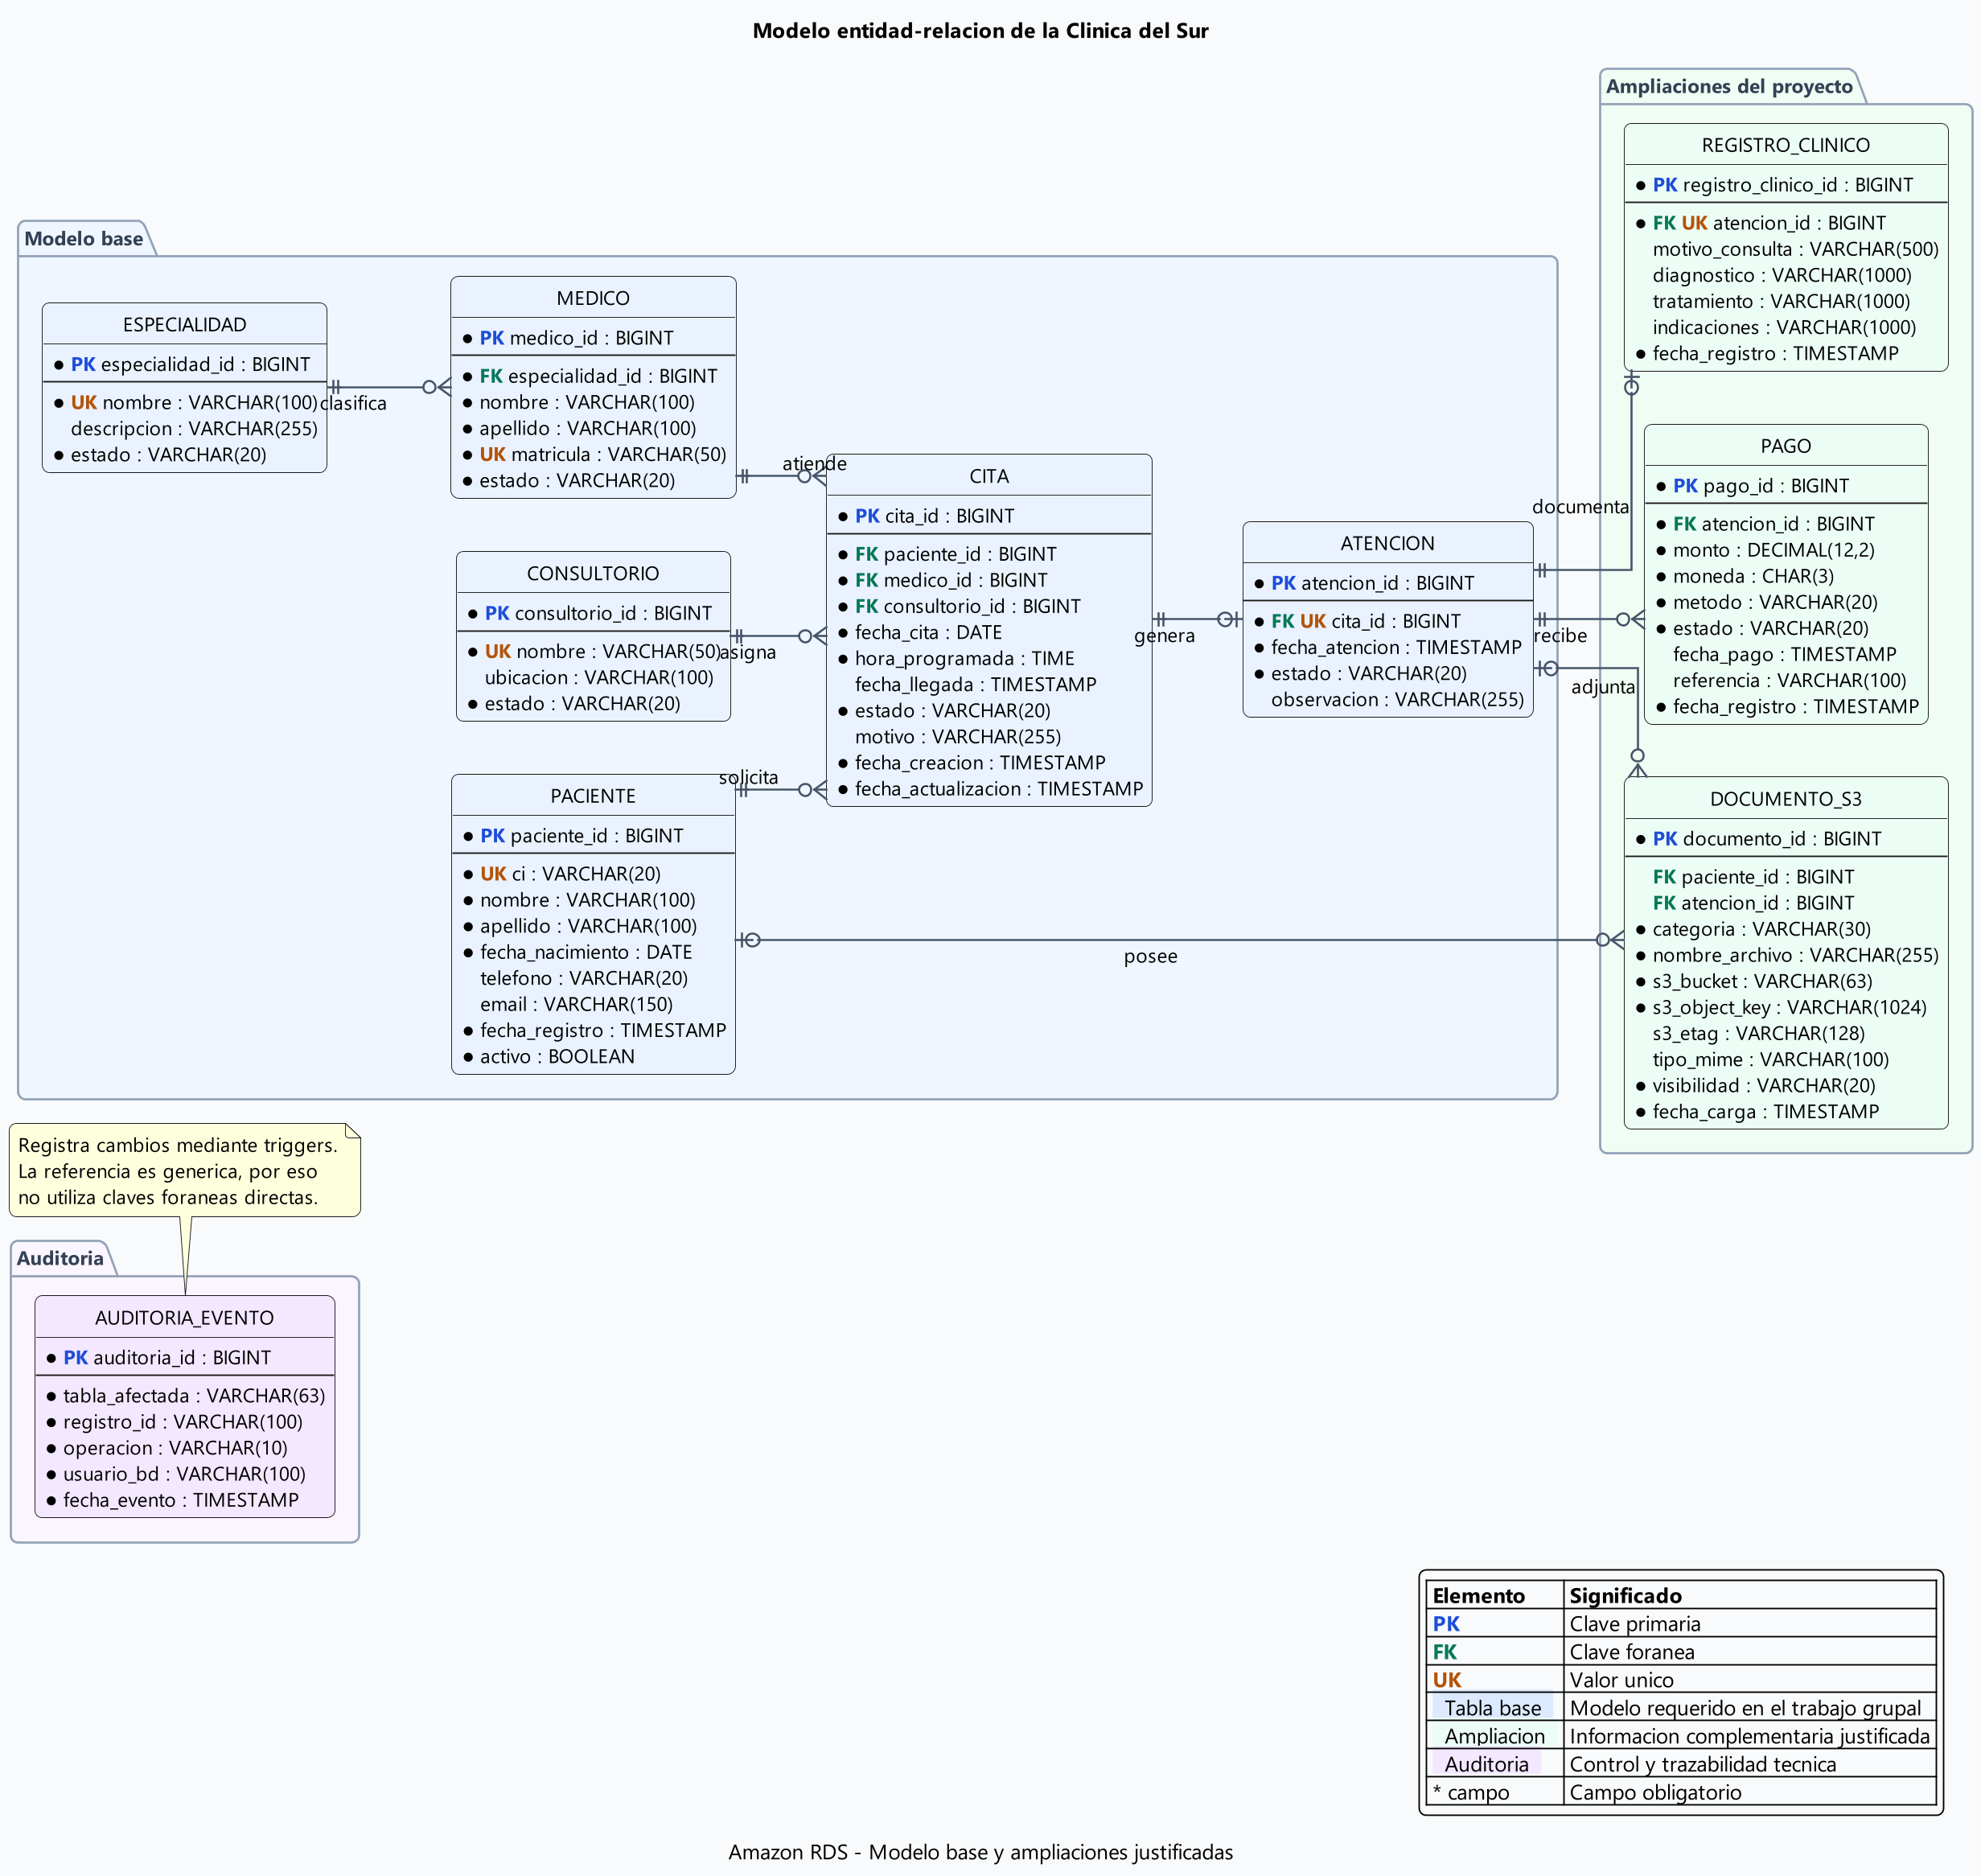
\includegraphics[width=\textwidth]{figures/modelo_datos_plantuml.png}
  \caption{Base de datos relacional de la clinica}
\end{figure}


\subsection{Datos de RDS utilizados para los KPI}

Los KPI se calcularan a partir de los datos almacenados en las tablas de RDS. La relacion entre
cada indicador y sus datos principales es la siguiente:

\begin{center}
\small
\begin{tabularx}{\textwidth}{@{}p{5cm}Y@{}}
  \toprule
  \rowcolor{azulclaro}
  \textbf{KPI} & \textbf{Datos principales de RDS} \\
  \midrule
  Pacientes atendidos por mes & PACIENTE.paciente\_id, ATENCION.fecha\_atencion y ATENCION.estado. \\
  Porcentaje de citas canceladas & CITA.cita\_id y CITA.estado. \\
  Atenciones por especialidad & ESPECIALIDAD.especialidad\_id, MEDICO.especialidad\_id, CITA.medico\_id y ATENCION.cita\_id. \\
  \bottomrule
\end{tabularx}
\end{center}

\section{S3 y analisis de informacion}

\subsection{Informacion que se almacenara en Amazon S3}

Amazon S3 se utilizara para almacenar los archivos y documentos no estructurados generados por la
Clinica del Sur. De esta manera, se mantendran separados los datos estructurados de RDS y los
archivos de mayor tamano o de tipo documental.

\begin{itemize}
  \item Resultados de laboratorio en formato PDF.
  \item Recetas medicas.
  \item Informes medicos.
  \item Imagenes de estudios medicos.
  \item Reportes mensuales de la clinica.
  \item Archivos del sitio web estatico de la clinica.
\end{itemize}

Los datos estructurados, como pacientes, medicos, especialidades, consultorios, citas y
atenciones, permaneceran en Amazon RDS. S3 complementara esta informacion almacenando los
documentos y archivos relacionados con la atencion de los pacientes.

Por ejemplo, RDS puede almacenar el registro de una atencion y S3 el informe medico o el resultado
de laboratorio asociado. Los reportes generados a partir de los KPI tambien podran guardarse en
S3 para su consulta historica.

\subsection{KPI de la clinica}

Los siguientes KPI fueron definidos de acuerdo con las necesidades planteadas en el punto 1 y se
calcularan utilizando los datos estructurados almacenados en Amazon RDS.

\begin{center}
\scriptsize
\begin{tabularx}{\textwidth}{@{}p{2.5cm}Y Y Y p{2.4cm}@{}}
  \toprule
  \rowcolor{azulclaro}
  \textbf{KPI} & \textbf{Que mide} & \textbf{Datos necesarios} & \textbf{Formula} & \textbf{Fuente} \\
  \midrule
  Pacientes atendidos por mes & Cantidad de pacientes que recibieron atencion durante un mes. & Paciente, fecha de atencion y estado. & Total de pacientes con atenciones completadas en el mes. & Amazon RDS: PACIENTE y ATENCION. \\
  Porcentaje de citas canceladas & Proporcion de citas programadas que fueron canceladas. & Total de citas y estado de la cita. & Citas canceladas / total de citas $\times 100$. & Amazon RDS: CITA. \\
  Atenciones por especialidad & Cantidad de atenciones realizadas en cada especialidad para identificar la mayor demanda. & Especialidad, medico, cita y atencion. & Total de atenciones agrupadas por especialidad. & Amazon RDS: ESPECIALIDAD, MEDICO, CITA y ATENCION. \\
  \bottomrule
\end{tabularx}
\end{center}

\subsection{Uso de los KPI}

Los KPI permitiran obtener informacion concreta sobre el funcionamiento de la clinica y apoyar la
toma de decisiones:

\begin{itemize}
  \item \textbf{Pacientes atendidos por mes:} permite conocer la cantidad de pacientes atendidos y observar su evolucion en el tiempo.
  \item \textbf{Porcentaje de citas canceladas:} ayuda a identificar problemas en la gestion de citas y evaluar acciones orientadas a disminuir las cancelaciones.
  \item \textbf{Atenciones por especialidad:} permite identificar las especialidades con mayor demanda y apoyar una mejor distribucion de medicos, consultorios y recursos.
\end{itemize}

Los resultados podran presentarse en reportes periodicos y almacenarse en Amazon S3, facilitando
su consulta historica y su uso posterior en el analisis de la clinica.

\section{IAM y arquitectura}

\subsection{Usuarios, roles y permisos mediante AWS IAM}

Los permisos siguen el principio de minimo privilegio: cada rol accede solamente a los recursos
necesarios para cumplir su responsabilidad.

\begin{table}[htbp]
  \centering
  \small
  \caption{Matriz basica de roles y permisos}
  \begin{tabularx}{\textwidth}{@{}p{3.1cm}Y Y@{}}
    \toprule
    \rowcolor{verdeclaro}
    \textbf{Rol} & \textbf{Acceso permitido} & \textbf{Restricciones} \\
    \midrule
    Medico & Consulta de informacion clinica, pacientes y citas; lectura de archivos medicos previamente autorizados en S3. & Sin administracion de infraestructura. \\
    Recepcionista & Registro de pacientes y gestion de citas. & Sin acceso a historias clinicas. \\
    Analista de datos & Consulta de la informacion necesaria para KPI y acceso a reportes historicos. & Sin modificacion de los registros operativos. \\
    Administrador TI & Administracion de buckets, configuracion, usuarios, roles, permisos, RDS y S3. & Acceso administrativo sujeto al principio de minimo privilegio. \\
    \bottomrule
  \end{tabularx}
\end{table}

% IMAGEN PENDIENTE: insertar una captura de los roles IAM despues de ocultar
% el identificador de cuenta y cualquier otro dato sensible.
% Archivo sugerido: latex-workshop/figures/roles_iam.png
% \includegraphics[width=\textwidth]{figures/roles_iam.png}

\subsection{Integracion de IAM, RDS y S3}

\begin{figure}[htbp]
  \centering
  \begin{tikzpicture}[
    node distance=7mm and 7mm,
    caja/.style={draw=grisborde, rounded corners=3pt, minimum height=1.2cm,
      minimum width=2.55cm, align=center, font=\small, fill=white},
    nucleo/.style={caja, draw=azulaws, fill=azulclaro},
    soporte/.style={caja, draw=verdeclinica, fill=verdeclaro},
    flecha/.style={-{Latex[length=2.2mm]}, thick, draw=gristexto}
  ]
    \node[nucleo] (usuarios) {Usuarios\\de la clinica};
    \node[nucleo, right=of usuarios] (iam) {AWS IAM\\roles y permisos};
    \node[nucleo, right=of iam, yshift=8mm] (rds) {Amazon RDS\\MySQL};
    \node[soporte, right=of iam, yshift=-8mm] (s3) {Amazon S3\\privado y web};
    \node[nucleo, right=of rds, yshift=-8mm] (analisis) {Consultas y\\calculo de KPI};
    \node[soporte, right=of analisis] (decision) {OKR y toma\\de decisiones};

    \draw[flecha] (usuarios) -- (iam);
    \draw[flecha] (iam) -- (rds);
    \draw[flecha] (iam) -- (s3);
    \draw[flecha] (rds) -- (analisis);
    \draw[flecha] (s3) -- (analisis);
    \draw[flecha] (analisis) -- (decision);
  \end{tikzpicture}
  \caption{Flujo general de la arquitectura AWS propuesta}
\end{figure}

Los usuarios se autentican y reciben permisos mediante IAM. Las operaciones estructuradas se
registran en RDS, mientras que S3 conserva documentos, imagenes y reportes. Las consultas sobre
RDS alimentan los KPI; los resultados permiten evaluar el OKR y orientar decisiones sobre citas,
personal y especialidades.

\subsection{Sitio web estatico en Amazon S3}

El grupo preparara y publicara un sitio web estatico en Amazon S3 para presentar el caso de
negocio, la arquitectura y los indicadores. El sitio no contendra historias clinicas ni datos
personales; los documentos medicos permaneceran en almacenamiento privado y solamente podran ser
consultados por roles autorizados.

\section{OKR}

\subsection{Objetivo}

\textbf{Objetivo:} Centralizar y organizar los datos generados por la clinica mediante una
arquitectura de datos en AWS, con el proposito de facilitar el analisis de las citas y los
servicios medicos, mejorar su gestion y apoyar la toma de decisiones.

\subsection{Key Results}

\begin{itemize}
  \item \textbf{KR1:} Reducir en 15\% las citas canceladas o no atendidas.
  \item \textbf{KR2:} Reducir en 10\% el tiempo promedio de espera de los pacientes.
  \item \textbf{KR3:} Incrementar en 10\% la cantidad de pacientes recurrentes.
\end{itemize}

\subsection{Relacion entre los datos, los KPI y el OKR}

El KR1 se evalua mediante los estados \emph{CANCELADA} y \emph{NO\_ATENDIDA} de la cita. El KR3
identifica pacientes atendidos que ya contaban con una atencion completada en un periodo anterior.
El modelo base permite calcular el retraso respecto de la hora programada comparando
\texttt{ATENCION.fecha\_atencion} con \texttt{CITA.fecha\_cita} y
\texttt{CITA.hora\_programada}. Para medir el tiempo real de espera desde la llegada del paciente,
se requiere agregar \texttt{CITA.fecha\_llegada}; este campo se considera una ampliacion tecnica y
debe ser aprobado por el grupo antes de incorporarlo al modelo base.

\section{Conclusion}

La arquitectura propuesta integra estrategia, datos y servicios AWS en un flujo verificable.
Amazon RDS organiza las operaciones y garantiza sus relaciones; Amazon S3 conserva archivos y
reportes con separacion entre contenido publico y privado; AWS IAM limita el acceso de acuerdo con
las responsabilidades del personal. Los KPI permiten observar demanda, cancelaciones y actividad
por especialidad, mientras que el OKR convierte esos indicadores en metas operativas. En conjunto,
la solucion mejora la disponibilidad de informacion y respalda decisiones sobre recursos,
programacion de citas y calidad de atencion.

\end{document}
